\documentclass[12pt, a4paper]{article}
\renewcommand*\contentsname{Inhaltsverzeichnis}
\usepackage[ngerman]{babel}
\usepackage{mathptmx}
\usepackage{blindtext}
\usepackage{emptypage}
\usepackage{wrapfig}
\usepackage[pdftex]{graphicx}
\usepackage{geometry}
\usepackage{setspace}
\usepackage{hyperref}
\usepackage[version=4,arrows=pgf-filled,
textfontname=sffamily,
mathfontname=mathsf]{mhchem}
\usepackage[table]{xcolor}
\usepackage{multirow}
\usepackage[table]{xcolor}
\usepackage{array}
\usepackage{float}
\usepackage{mathcomp}
\usepackage{csquotes}
\usepackage[backend=biber,style=chem-acs,sorting=none]{biblatex}
\addbibresource{literatur.bib}  % Deine .bib-Datei einbinden
\renewcommand{\thefootnote}{\fnsymbol{footnote}}

\DeclareCiteCommand{\cite}
  {\usebibmacro{prenote}}
  {\textsuperscript{\printfield{labelnumber}}}
  {\multicitedelim}
  {\usebibmacro{postnote}}


 \geometry{
 a4paper,
 total={170mm,257mm},
 left=25mm,
 top=25mm,
 }
\setstretch{1.213}


\newcommand{\datum}{\day.\month.\year}
\DeclareGraphicsExtensions{.pdf,.jpeg,.png,.jpg} 

\begin{document}


\begin{figure}
    \includegraphics[scale=0.14]{Universität_Bayreuth.svg.png}
\end{figure}


%Deckblatt

{\raggedright Universität Bayreuth\\  95447 Bayreuth}


\vspace{5cm}

\begin{center}
{\LARGE\bf{Anorganische Chemie III}} \\  
\vspace{1cm}
{\Large\bf{Magnetphasen}}\\
\vspace{0.5cm}
{\large Justus Friedrich\\}
{Studiengang: B.Sc. Chemie\\}
{4. Fachsemester}
\end{center}





\thispagestyle{empty}
\begin{center}
{\small Matrikelnummer: 1956010 \\
E–Mail:  bt725206@myubt.de}
\end{center}

\vspace{5cm}

\today


\newpage
%Inhaltsverzeichnis
\tableofcontents
\thispagestyle{empty}


%Teil 1
\newpage
\setcounter{page}{1}
\section{Einleitung}



\subsection{Einführung}


{Magnetismus ist eine Eigenschaft, die auf der Anordnung der Elektronenspins beruht. Diese Spins erzeugen ein magnetisches Moment. Wenn sich die magnetischen Momente innerhalb
 eines Atoms gegenseitig aufheben, ist der Stoff diamagnetisch. Besitzt ein Atom hingegen ein resultierendes magnetisches Moment, ist der Stoff paramagnetisch.\\
\noindent
Paramagnetische Stoffe lassen sich weiter in Ferromagnete, Ferrimagnete und Antiferromagnete unterteilen:
\begin{enumerate}
    \item Bei Ferromagneten richten sich alle magnetischen Momente parallel zueinander aus, wodurch ein starkes makroskopisches Magnetfeld entsteht.
    \item Bei Ferrimagneten sind die magnetischen Momente zwar auch geordnet, jedoch in entgegengesetzten Richtungen mit unterschiedlicher Stärke ausgerichtet. Dadurch bleibt ein resultierendes magnetisches Moment bestehen, das jedoch schwächer ist als bei Ferromagneten.
    \item In Antiferromagneten sind die magnetischen Momente benachbarter Atome entgegengesetzt und gleich stark ausgerichtet, wodurch sie sich gegenseitig vollständig aufheben. Das resultierende magnetische Moment ist somit nazu null.
\end{enumerate}
\noindent
Ziel des Versuchs ist es, Magnetit, Maghemit und Hämatit herzustellen und ihre magnetischen Eigenschaften zu untersuchen. \cite{Skript}
}


\newpage
%Teil2
\section{Durchführung}
\subsection{Darstellung von Magnetit}
Es werden 3.001 g (15.09 mmol) \ce{FeCl2}$\cdot$\ce{4 H2O} in 75 mL Wasser gelöst. Anschließend wird 30 mL einer 1 Molarer (2.599 g/ 65mmol in 65 mL Wasser) NaOH
unter kräftigen Rühren hinzugegeben. Nach 35 min wird der Niederschlag abgenutscht und getrocknet.

\subsection{Darstellung von Maghemit}
Ein Teil des Hergestellten Magnetits wird für 2 h bei 250 °C getempert.

\subsection{Darstellung von Hämatit}
Ein Teil des Maghemit wird für 10 h bei 700°C getempert.\footnote{Hier sollte eigentlich nur für 2 h getempert werden, aufgrund eines Fehlers wurde für 10 h getempert.}


\newpage
\section{Auswertung}
\subsection{Phasenanalyse von Magnetit}

Da bei der verwendeten Wellenlänge der Röntgenquelle eine starke Fluoreszenz von Eisen auftritt, konnten keine eigenen XRD-Messungen an den hergestellten Substanzen durchgeführt werden. 
Um dennoch eine Vergleichsbasis zur Interpretation zu schaffen, wurde ein Referenzdiffraktogramm von Magnetit herangezogen.
Die Beispielmessung ist in Abbildung \Ref{Magnetitxrd} dargestellt. 

\noindent
Bei der Analyse der XRD-Daten zeigte sich eine Vertauschung der Dateinamen: Die Datei „Magnetit“ enthält das Diffraktogramm von Maghemit, und „Maghemit“ jenes von Magnetit. Diese Verwechslung wurde im Protokoll berücksichtigt, sodass die Dateien im Folgenden entsprechend korrigiert zugeordnet werden.
\begin{figure}[!h]
    \centering
    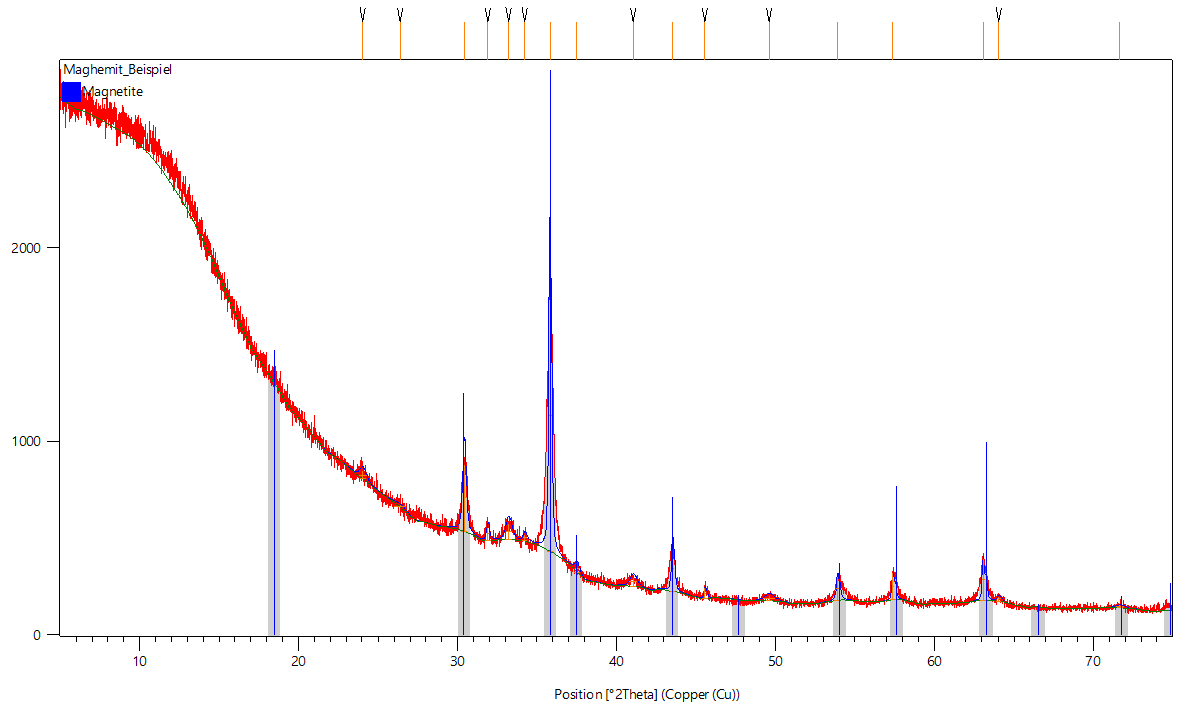
\includegraphics[width=0.8\linewidth]{Magnetit.png}
    \caption{Das XRD-Diagramm zeigt Magnetit mit den Referenzreflexen gemäß dem Referenzcode 01-075-0449.}
    \label{Magnetitxrd}
\end{figure}

\noindent
Als Hauptphase wurde mit 67 \% kubisches Magnetit identifiziert (\textit{HighScore Plus} Score 54, Referenzcode 01-075-0449); als Nebenphase wurde mit 33 \% rhomboedrisches \ce{Fe2O3} bestimmt (\textit{HighScore Plus} Score 17, Referenzcode 01-073-2234).
Anschließend wird die Theoretische Elementarzelle mit der Festgestellten Elementarzelle verglichen. Dies wird in der Tabelle \ref{Kastenlängemagnetit} dargestellt.
\newpage
\begin{table}[h!]
\caption{\textit{Zeigt die Theoretische (Referenzcode 01-075-0449) und Festgestellte verfeinerte Einheitszelle von den hergestellten Magnetit. Die Verfeinerung wurde mithilfe des Programmes HighScore Plus durchgeführt. }}
\begin{center}
\begin{tabular}{|>{\columncolor{lightgray}}p{4cm}|>{\centering\arraybackslash}p{4cm}|>{\centering\arraybackslash}p{4cm}|}
   \hline
   \rowcolor{gray}
   &Theoretische Elementarzelle& Festgestellte verfeinerte Elementarzelle (Standardabweichung) \\
   \hline
   a[\AA]& 8.3100& 8.324 (3)\\
   \hline
   b[\AA]&8.3100& 8.324 (3)\\
   \hline
   c[\AA]&8.3100& 8.324 (3)\\
   \hline
   $\alpha$[°]&90& 90\\
   \hline
   $\beta$[°]&90& 90\\
   \hline
   $\gamma$[°]&90& 90\\
   \hline
   Volumen[\AA$^3$]&573.86 & 576.68\\
   \hline
    Chi Square&\multicolumn{2}{c|}{4.270028 $\cdot 10^{-6}$}\\
   \hline
   Synder`s FOM&\multicolumn{2}{c|}{9.4929}\\
\hline
\end{tabular}
\label{Kastenlängemagnetit}
\end{center}
\end{table}

\noindent
Aus Tabelle \ref{Kastenlängemagnetit} lässt sich erkennen, dass die Elementarzellen nicht vollständig übereinstimmen. Dies liegt wahrscheinlich an der \ce{Fe2O3}-Verunreinigung.

\subsection{Phasenanalyse von Maghemit}
Das exemplarische XRD wird in der Abbildung \ref{maghemitxrddd} dargestellt.

\begin{figure}[!h]
    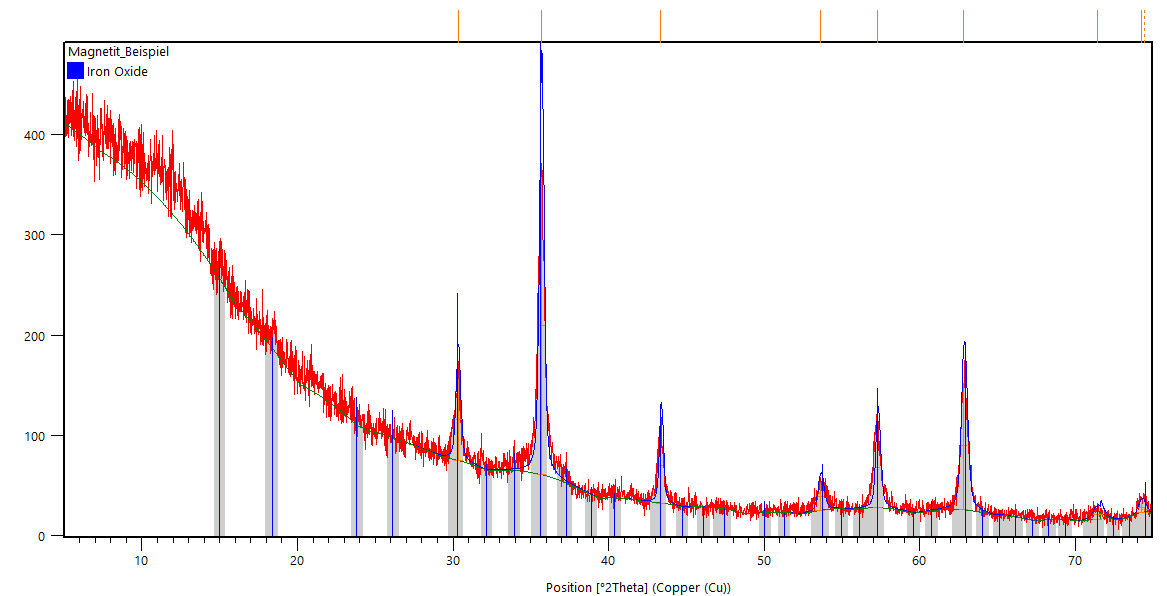
\includegraphics[width=\linewidth]{Magnehit.png}
    \caption{Zeigt das XRD vom Maghemit mit Referenzreflexen mit den Referenzcode 01-083-0112}
    \label{maghemitxrddd}
\end{figure}

Das XRD, aus Abbildung \ref{maghemitxrddd}, zeigt Maghemit (Score 66, 75 \%) und Referenzreflexe mit den Referenzcode 01-083-0112, außerdem lässt sich Magnetit (Score 30, 25 \%) als Phase feststellen.
Anschließend wird wieder die Elementarzelle betrachtet. Dies wird in der Tabelle \ref{Kastenlängemaghemit} dargestellt.

\begin{table}[h!]
\caption{\textit{Zeigt die Theoretische (Referenzcode 01-083-0112) und Festgestellte verfeinerte Einheitszelle von den hergestellten Maghemit. Die Verfeinerung wurde mithilfe des Programmes HighScore Plus durchgeführt. }}
\begin{center}
\begin{tabular}{|>{\columncolor{lightgray}}p{4cm}|>{\centering\arraybackslash}p{4cm}|>{\centering\arraybackslash}p{4cm}|}
   \hline
   \rowcolor{gray}
   &Theoretische Elementarzelle& Festgestellte verfeinerte Elementarzelle (Standardabweichung) \\
   \hline
   a[\AA]& 8.3474 & 8.358 (4)\\
   \hline
   b[\AA]&8.3474& 8.358 (4)\\
   \hline
   c[\AA]&8.3474& 8.358 (4)\\
   \hline
   $\alpha$[°]&90& 90\\
   \hline
   $\beta$[°]&90& 90\\
   \hline
   $\gamma$[°]&90& 90\\
   \hline
   Volumen[\AA$^3$]&581.64 & 583.87\\
   \hline
    Chi Square&\multicolumn{2}{c|}{7.359962 $\cdot 10^{-6}$}\\
   \hline
   Synder`s FOM&\multicolumn{2}{c|}{2.3284}\\
\hline
\end{tabular}
\label{Kastenlängemaghemit}
\end{center}
\end{table}

\noindent
Auch hier lassen sich kleine Abweichungen von der theoretischen Elementarzelle beobachten. Diese resultieren daraus, dass in der Probe noch Magnetit vorhanden ist. Da die Probe nicht im Rahmen des Praktikums hergestellt wurde, lässt sich keine Aussage darüber treffen, wie der Magnetit-Anteil reduziert werden könnte.



\newpage



\subsection{Magnetit-Anteil Bestimmung in einer Maghemit-Probe}
Um den Magnetit-Anteil bestimmen zu können, wird zunächst die Elementarzelle bestimmt. Dazu werden in Abbildung \ref{maghemitxrddd2} zunächst die Reflexe den Referenzreflexen (Referenzcode 01-083-0112) zugeordnet. Anschließend wird die Elementarzelle ermittelt und in Tabelle \ref{Kastenlängemaghemit2} eingetragen.

\begin{figure}[!h]
    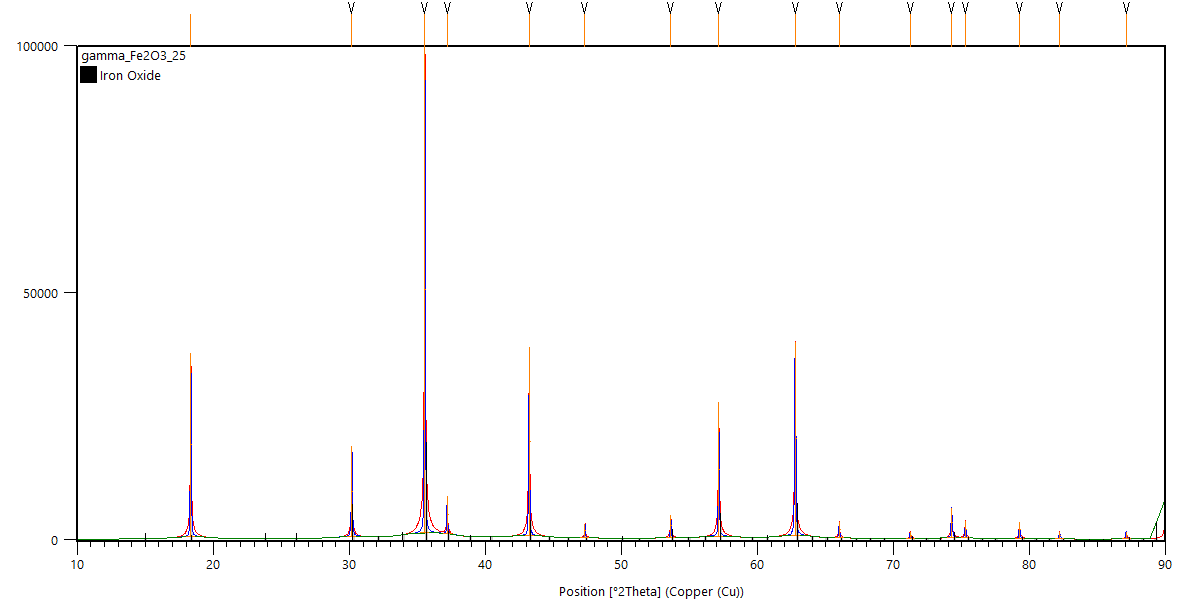
\includegraphics[width=\linewidth]{Maghemit.png}
    \caption{Zeigt das XRD vom Maghemit mit Referenzreflexen mit den Referenzcode 01-083-0112}
    \label{maghemitxrddd2}
\end{figure}
\noindent
Auch hier ist von \textit{HighScore Plus} Magnetit (Referenzcode 01-074-1909) als Fremdphase identifiziert worden.
\begin{table}[h!]
\caption{\textit{Zeigt die Theoretische (Referenzcode 01-083-0112) und Festgestellte verfeinerte Einheitszelle von den hergestellten Maghemit. Die Verfeinerung wurde mithilfe des Programmes HighScore Plus durchgeführt. }}
\begin{center}
\begin{tabular}{|>{\columncolor{lightgray}}p{4cm}|>{\centering\arraybackslash}p{4cm}|>{\centering\arraybackslash}p{4cm}|}
   \hline
   \rowcolor{gray}
   &Theoretische Elementarzelle& Festgestellte verfeinerte Elementarzelle (Standardabweichung) \\
   \hline
   a[\AA]& 8.3474 & 8.368 (3)\\
   \hline
   b[\AA]&8.3474& 8.368 (3)\\
   \hline
   c[\AA]&8.3474& 8.368 (3)\\
   \hline
   $\alpha$[°]&90& 90\\
   \hline
   $\beta$[°]&90& 90\\
   \hline
   $\gamma$[°]&90& 90\\
   \hline
   Volumen[\AA$^3$]&581.64 & 585.96\\
   \hline
    Chi Square&\multicolumn{2}{c|}{3.408849 $\cdot 10^{-11}$}\\
   \hline
   Synder`s FOM&\multicolumn{2}{c|}{2213.4990}\\
\hline
\end{tabular}
\label{Kastenlängemaghemit2}
\end{center}
\end{table}

\noindent
Der Magnetit-Anteil lässt sich nun anhand der Größe der Elementarzelle bestimmen, denn je größer die Elementarzelle ist, desto höher ist der Magnetit-Gehalt in der Probe. Dies liegt daran, dass vermehrt Eisen(II) in die Kristallstruktur eingebaut wird. Der Zusammenhang ist in Abbildung \ref{diagramm} dargestellt.

\begin{figure}[!h]
    \centering
    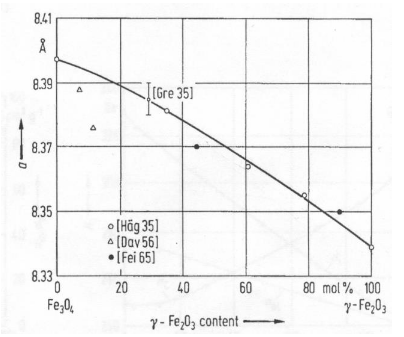
\includegraphics{diagramm.png}
    \caption{Diagramm, dass den Zusammenhang vom Magnetit-Anteil zur Elementarzellengröße zeigt.}
    \label{diagramm}
\end{figure}

\noindent
Daraus folgt, dass die Maghemit-Probe etwa aus 55 \% Maghemit und 45 \% Magnetit besteht. Die Probe aus Abschnitt 3.2 setzt sich aus ungefähr 70 \% Maghemit und 30 \% Magnetit zusammen.
Der Anteil von Maghemit lässt sich durch eine vollständigere Oxidation erhöhen. Dies kann durch längeres Tempern erreicht werden, da dadurch mehr Zeit zur vollständigen Oxidation zur Verfügung steht.

\newpage

\subsection{Hämatit}
Das XRD von Hämatit ist in Abbildung \ref{xrdhämatit} abgebildet.

\begin{figure}[!h]
    \includegraphics[width=\linewidth]{Hämatit.png}
    \caption{Zeigt das XRD von Hämatit mit Referenzreflexen (Referenzcode 00-013-0534)}
    \label{xrdhämatit}
\end{figure}

\noindent
Im XRD lässt sich als Hauptphase mit 97 \% Hämatit (Score 83, Referenzcode 00-013-0534) feststellen. Als Nebenphase wurde mit 3 \% Wüstit (Score 17, Referenzcode 01-079-1967) identifiziert. Die genaue Ursache für die Bildung von Wüstit ist nicht bekannt. Anschließend wird erneut die Elementarzelle bestimmt.
Diese wird in der Tabelle 


\begin{table}[h!]
\caption{\textit{Zeigt die Theoretische (Referenzcode 00-013-0534) und Festgestellte verfeinerte Einheitszelle von den Hämatit. Die Verfeinerung wurde mithilfe des Programmes HighScore Plus durchgeführt. }}
\begin{center}
\begin{tabular}{|>{\columncolor{lightgray}}p{4cm}|>{\centering\arraybackslash}p{4cm}|>{\centering\arraybackslash}p{4cm}|}
   \hline
   \rowcolor{gray}
   &Theoretische Elementarzelle& Festgestellte verfeinerte Elementarzelle (Standardabweichung) \\
   \hline
   a[\AA]&  5.4228 & 5.39 (3)\\
   \hline
   b[\AA]&5.4228& 5.39 (3)\\
   \hline
   c[\AA]&5.4228& 5.43 (3)\\
   \hline
   $\alpha$[°]&90& 90\\
   \hline
   $\beta$[°]&90& 90\\
   \hline
   $\gamma$[°]&90& 90\\
   \hline
   Volumen[\AA$^3$]&138.10 & 136.77\\
   \hline
    Chi Square&\multicolumn{2}{c|}{2.231119 $\cdot 10^{-4}$}\\
   \hline
   Synder`s FOM&\multicolumn{2}{c|}{2.3612}\\
\hline
\end{tabular}
\label{Kastenlängehämatit}
\end{center}
\end{table}
\noindent
Auch in diesem Fall zeigen die ermittelten Parameter eine gute Übereinstimmung mit der Referenz, wobei die beobachtete Struktur eine leichte Verzerrung aufweist.

\subsection{Test des Magentischen Verhaltens}

Um zu testen, ob die hergestellten Eisenoxide von einem Magnetfeld beeinflusst werden, werden sie auf einen Magneten gestellt. Dies ist in Abbildung \ref{testmagnet} dargestellt.
\begin{figure}[!h]
    \centering
    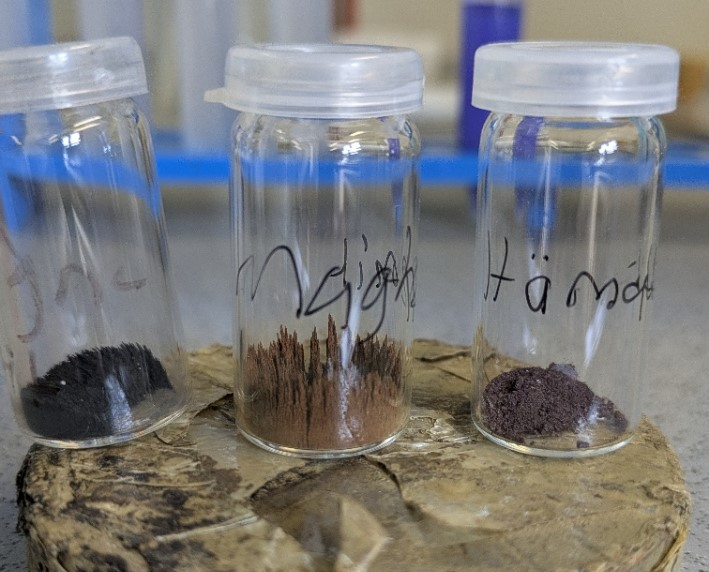
\includegraphics[width=0.5\linewidth]{testmagnet.jpg}
    \caption{Zeigt Magnetit (Links), Maghemit (Mitte) und Hämatit (Rechts) auf einem Magneten.}
    \label{testmagnet}
\end{figure}

\noindent
Es ist zu erwarten, dass sowohl Magnetit als auch Maghemit als Ferrimagnete vom Magnetfeld beeinflusst werden. Hämatit hingegen sollte nicht beeinflusst werden, da es sich um einen Antiferromagneten handelt. Diese Erwartung wurde im Versuch bestätigt, siehe Abbildung \ref{testmagnet}, sodass davon ausgegangen werden kann, dass die Synthese erfolgreich war.

\newpage

\section{Zusatzfragen}
\subsection{Präzipitationsmethode}
Ein Nachteil der Präzipitationsmethode besteht darin, dass die Partikelgröße nur schwer genau kontrolliert werden kann. Dadurch entsteht oft eine breite Größenverteilung der Partikel. Für den Superparamagnetismus ist jedoch eine eng definierte Partikelgröße notwendig, da nur sehr kleine Nanopartikel ($<$ ca. 20 nm) dieses Verhalten zeigen.
Trotzdem lässt sich die Partikelgröße beeinflussen, indem die Reaktionsbedingungen gezielt gesteuert werden. Eine effektive Maßnahme ist beispielsweise die langsame Zugabe der Reaktanden, um die Nukleation und das Kristallwachstum besser kontrollieren zu können.

\subsection{Permanentmagneten}
Maghemit eignet sich am besten für Permanentmagneten, weil es ferrimagnetisch ist, eine hohe Koerzitivfeldstärke hat und gegen Oxidation stabil ist.
Eine dauerhafte Magnetisierung entsteht, wenn das Material in einem starken Magnetfeld magnetisiert wird und durch Kompaktierung oder Strukturierung so stabil ist, dass sich die magnetischen Momente nicht leicht umdrehen lassen.
\subsection{Kristallstrukturen}
Magnetit besitzt eine inverse Spinellstruktur, in der \ce{Fe^{3+}}-Ionen sowohl die Oktaeder- als auch Tetraederpositionen besetzen, während \ce{Fe^{2+}}-Ionen ausschließlich in den Oktaederpositionen vorliegen.

\noindent
Maghemit besitzt eine ähnliche kubische Struktur wie Magnetit, enthält jedoch ausschließlich \ce{Fe^{3+}}-Ionen, dies führt zu strukturellen Leerstellen zum Ladungsausgleichung welches zu einer verzerrten Strucktur führt.

\noindent
Hämatit kristallisiert in einer rhomboedrischen Struktur. Die Sauerstoffanionen bilden eine hexagonal dichteste Packung, in der zwei Drittel der Oktaederlücken mit \ce{Fe^{3+}}-Ionen besetzt sind.

\newpage
\section{Zusammenfassung}
Im Versuch konnten erfolgreich Magnetit, Maghemit und Hämatit synthetisiert werden. Da jedoch keine eigenen Pulverdiffraktogramme aufgenommen werden konnten, wurde auf Beispielmessungen zurückgegriffen.

\noindent
Bei der Auswertung stellte sich heraus, dass in den Proben von Magnetit und Maghemit jeweils Anteile der jeweils anderen Phase vorhanden sind. In der Hämatit-Probe wurde Wüstit als Fremdphase identifiziert.

\noindent
In den ausgewerteten Pulverdiffraktogrammen von Maghemit konnte ein Anteil an Magnetit nachgewiesen werden. Die quantitative Phasenanalyse ergab, dass in einer Probe 55 \% Maghemit und in der anderen 70 \% Maghemit enthalten waren. Der Rest entfiel jeweils auf Magnetit als Nebenphase.


\newpage
\section{Literaturverzeichnis}
\printbibliography







\end{document}